\documentclass[12pt,letter]{article}

%compile with pdflatex:
%:! bibtex %:r
%:! pdflatex -synctex=1 -interaction=nonstopmode --shell-escape %

\usepackage{amsmath}
\usepackage{natbib}
\usepackage{graphicx}
\usepackage{hyperref}
\usepackage{booktabs}
\newcommand{\tabitem}{~~\llap{\textbullet}~~}

\usepackage{gnuplottex}
\usepackage{subcaption}
\usepackage{caption}
\captionsetup{font={sf,small},labelfont=bf,width=0.95\textwidth}
%\usepackage{wrapfig}
\usepackage{multirow}
\newcommand{\tabitem}{~~\llap{\textbullet}~~}

\title{Benchmark Validation and Bayesian Analysis of Lava Flow Model Performance}
%\date{}
%\author{Jacob Richardson, Laura Connor\\ Charles Connor, Sylvain Charbonnier}
\author{Jacob Richardson}

\usepackage[margin=1in]{geometry}
\usepackage{setspace}
%\doublespacing

%\usepackage{lineno}
%\linenumbers

\usepackage{titlesec}
\titleformat*{\section}{\large\bfseries} %LARGE, Large, large
\titleformat*{\subsection}{\normalsize\bfseries} %LARGE, Large, large

%Geology Papers are limited to ~5000 words

\begin{document}

\maketitle

\section*{Abstract}
	Modeling lava flows through cellular automata (CA) methods enables a computationally inexpensive means to quickly forecast lava flow paths and ultimate areal extents. A CA program has been created in the program language C that is modular, which enables a combination of governing CA rules to be evaluated against each other. My objective is to find a successful combination of automata behaviors that accurately forecasts lava inundation and behaves like a bingham fluid. To fulfill this objective, four benchmarking levels have been devised to test lava spreading algorithms against increasingly complex tests. These levels are 1) verification of the code by testing for conservation of mass; 2) testing for flow self-similarity given inconsequential variations of arbitrary surfaces; 3) testing for replication of Bingham flow morphology on simple surfaces and; 4) testing for replication of real lava flow morphologies on pre-eruptive surface models. Currently the best-fitting lava spreading algorithm for these four benchmarking tests might be an algorithm which spreads lava proportional to slope and where each automaton is able to spread lava in 8 directions.

\section{Introduction}
	Lava flows as a gravity current on the surface of the Earth when liquid magma is effused at the surface with little or no explosivity. In the vacinity of active volcanoes, lava flows represent significant long term impact to infrastructure. In the past, lava flow hazard has been mitigated with the construction of physical diversions and at least once in 252 AD by the supernatural grace of St. Agatha of Sicily who died the year prior. Modern science suggests, however, that forecasting the flow path of lava from active volcanoes might be more useful than St. Agatha for communities impacted by effusive volcanism.

	Methods of forecasting lava flows range from simple predictions using empirical relationships between magma flux and flow length \citep{Glaze2003}, to 1-D numerical solutions such as FLOWGO \citep{harris2001flowgo}, to advanced computational fluid dynamics codes like lavaSIM \citep{hidaka2005vtfs}. All modern numerical flow models by nature trade precision in simulating physical processes with computer run-time, so that while FLOWGO is relatively fast it only predicts downslope flow length, while lavaSIM solves Navier-Stokes equations to produce a 3-D flow distribution at the expense of large computational requirements.
	
	Cellular Automata (CA) methods have been developed to simulate fluid flow, including lava spreading \citep{barca1994cellular}. In contrast to CFD codes, these do not generally attempt to compute Navier-Stokes equations but instead abstract many physical parameters, such as viscosity and temperature, into more or less empirical rules. The benefit of CA methods for simulating lava flows is most noticeable in the reduced computer time necessary for simulation compared to CFD methods.
	
	Multiple CA lava flow algorithms exist, such as SCIARA \citep{crisci2004simulation}, MAGFLOW \citep{del2008simulations}, ELFM \citep{damiani2006lava}, and LavaPL \citep{connor2012}. These algorithms are variations on a theme, where the largest difference between each is how lava is distributed from one automaton to its neighbors. For instance, three versions of SCIARA allow for lava to spread in cardinal directions \citep{barca1994cellular}, in hexagonal directions \citep{crisci2008lava}, or in directions based on an inherent velocity calculated in an eulerian way for each automaton \citep{avolio2006sciara}. MAGFLOW and ELFM by contrast to the original SCIARA algorithm implements 8 directions of spreading. LavaPL and SCIARA both spread in four directions but the apportionment of lava from one automaton to neighbors is based on a different algorithm.

	While several lava flow simulators now exist, each have been made and tested with different lava flows or aspects of flows in mind. Because of this, selecting a specific algorithm to effectively model lava flow hazards can be a necessary, if unwanted challenge. To address this problem, we propose a hierarchical benchmarking scheme to objectively rank different flow spreading algorithms. This hierarchy tests simulated output against increasingly complex tests, from simply conserving mass to replicating the paths and ultimate areal extents of real lava flows. These benchmarking methods can be applied to any flow algorithm that provides at least a list or map of inundated locations over various topographies.

	In this paper, multiple lava flow algorithms are tested using a new modular lava flow code, which I have named MOLASSES (standing for \textit{MOdular LAva Simulation Software in Earth Science}). This code, implemented in C, is a Cellular Automata code which tracks a population of equal-area spaced cells over a grid, that is defined by a digital elevation model (DEM). These cells may or may not be inundated with lava and they are governed by universal rules. Because MOLASSES has been designed in a modular way, it is relatively quick to modify the flow algorithm. Using this code while changing methods of lava distribution enables code output in a constant format, which simplifies the comparison of methods.
	
	In Section \ref{sec:MOLASSES}, I will demonstrate how CA is applied to lava flows and detail how a CA simulation is carried out in the MOLASSES code. I will introduce a hierarchy of benchmarks in Section \ref{sec:benchmark} that can be used to verify and validate different lava flow algorithms using increasingly complex model parameters. In Section \ref{sec:Bayesian}, I will expand on the final benchmark level (validation against real flows) with a Bayesian approach to improving model performance for the 2012-3 Tolbachik Lava Flow. The results from these Sections will be discussed in Section \ref{sec:discussion}.
	
	\subsection{Case Study Area: 2012-3 Tolbachik Lava Flow}\label{sec:tolb_back}
The Tolbachik lava flow began in November 2012, originally being sourced from a long fissure vent south of Tolbachik Dol. Initial magma flux was estimated to be 440~m$^3$~s$^{-1}$ \citep{belousov2015overview}. The fissure vent ultimately coalesced into two main vents, seen in TanDEM-X data and the flux dropped significantly to between 100 and 200~m$^3$~s$^{-1}$. Early stages of the flow carried lava west to a maximum runout of 14.5~km and later stages beginning in January or February, carried lava east. The total emplacement volume is $\sim$0.5~cu.~km. with 0.38~cu.~km. of that being to the west. TanDEM-X data show that the modal thickness of the flow is 7.8~m, and that the overall thickness distribution is log-normal. After the flow ceased, the total emplacement area was mapped using orthophotos and TanDEM-X data where clouds were present in the images by \citet{kubanek2015lava}.
	

%%%%%%%%%%%%%%%%%%%%%%%%%%%%%%%%%%%%%%%%%%%%%%%%%
%MOLASSES%%%%%%%%%%%%%%%%%%%%%%%%%%%%%%%%%%%%%%%%
%%%%%%%%%%%%%%%%%%%%%%%%%%%%%%%%%%%%%%%%%%%%%%%%%
%%%%%%%%%%%%%%%%%%%%%%%%%%%%%%%%%%%%%%%%%%%%%%%%%
%%%%%%%%%%%%%%%%%%%%%%%%%%%%%%%%%%%%%%%%%%%%%%%%%

\section{A Modular Cellular Automata Algorithm for lava flows}\label{sec:MOLASSES}

CA in lava flows has historically been defined as a 2-dimensional space, which is divided into equal-area grid cells, such as those found in a common digital elevation model (DEM). Within the location of each cell is defined an ``elementary automaton'' (\textit{ea}) that has a set of properties, is governed by a set of global rules, and has a set list of neighboring automata. While the behavior rules that each \textit{ea} follow is identical to those of all other automata, its behavior is only dictated by local phenomena. Specifically, the amount of lava that flows in or out of an \textit{ea} will depend on properties such as lava thickness and elevation within it and its neighbors. Because grid cells and \textit{ea} are fundamentally inseperable in this application, I will refer to \text{ea} as cells.

The set of cellular automata is defined as
	\begin{equation}
		\mathbf{A} = \mathrm{\{E^2, V, S, X, \sigma, \gamma\}}
	\end{equation}
	where E$^2$ is the set of point locations of cells in \textbf{A}, V$\subset$E$^2$ is the set of vent or source locations, S is the set of substates within each cell, and X is the local neighborhood that each cell can directly influence \citep{barca1994cellular}. $\sigma$ and $\gamma$ represent the transition functions and source functions within \textbf{A}. 
	
	Practically, E$^2$ is a set of coordinate pairs denoting row and column addresses of cells in a larger grid. S($i$,$j$), which represents the set of substates for the cell at row $i$, column $j$, includes S$_e$, the underlying elevation of an automaton; S$_h$, the thickness of lava within the cell; and S$_{h0}$, the critical thickness, above which lava will spread from a cell. Some algorithms include S$_T$, or the cell temperature in this set. X, in a four-connected neighborhood scheme, is given as \{(0,1), (0,-1), (1,0), (-1,0)\}, where (0,0) is the location of a cell under evaluation. $\sigma$ is the change of substates in S for each cell from timestep $t$ to $t+1$, or S$^{t}\rightarrow$S$^{t+1}$. $\gamma$ specifies the lava emitted at locations within V. The implementation of these sets within the CA structure \textbf{A} is described in detail below.
	
	\subsection{MOLASSES Algorithm Outline}
		MOLASSES is constructed with nine modules which each have a specific task, either carrying out the CA simulation, reading model input, or writing model output (Figure \ref{fig_flowchart}). The nine modules are:
		\begin{enumerate}
			\item{\textbf{DRIVER}} Calls modules in sequence to execute the flow algorithm.
			\item{\textbf{INITIALIZE}} Reads a user-provided configuration file to define model parameters.
			\item{\textbf{DEM\_LOADER}} Imports a raster file to define the elevation model.
			\item{\textbf{INITFLOW}} Uses model parameters to define data arrays.
			\item{\textbf{PULSE}} Incrementally adds lava to source locations.
			\item{\textbf{DISTRIBUTE}} Determines whether to spread and how to spread lava between cells.
			\item{\textbf{NEIGHBOR\_ID}} Identifies the cell neighborhood.
			\item{\textbf{ACTIVATE}} Adds newly inundated cells to the list of active cells.
			\item{\textbf{OUTPUT}} Writes model results to a file using user-specified formats.
		\end{enumerate}
		
		\begin{figure}[!h]
			\centering
			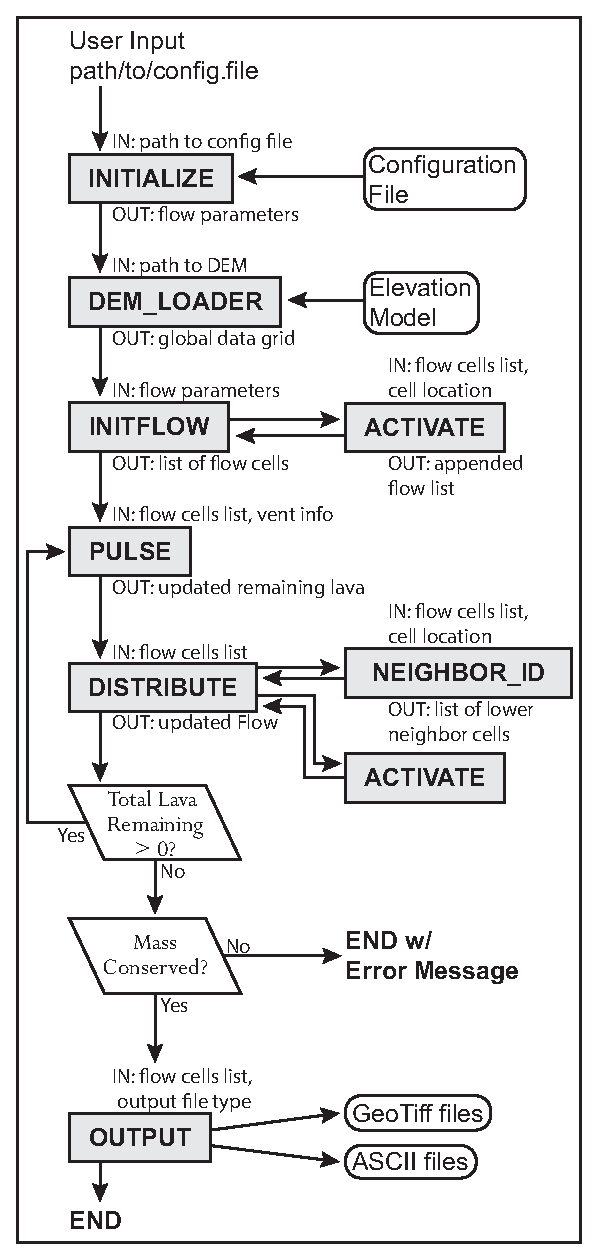
\includegraphics[width=0.2\linewidth]{figures/Flow_Chart}
			\caption{A flow chart of MOLASSES carried out within the \textbf{DRIVER} module.}
			\label{fig_flowchart}
		\end{figure}
		
		
		Model parameters are specified by a user through a text configuration file, which must include 1) a digital elevation model (DEM), 2) a residual lava flow thickness, 3) at least one vent location, 4) the total volume and ``pulse volume'' of this vent, and 5) an output file path. The lava flow thickness defines the CA value of S$_{h0}$, where cells with flow thicknesses S$_h>$S$_{h0}$ will spread all lava to their neighboring cells, while cells with less lava will retain their lava. The ``pulse volume'' defines $\gamma$ and the amount of lava to emit at the source location at each time step. The total volume constrains $\gamma$ as lava will not be introduced to the source location after the total volume has been delivered. Modules within MOLASSES that further execute the CA simulation are detailed below.
		
	\subsection[Cells in E2]{Cells in E$^2$}
		%DEM_LOADER
		%INITFLOW
		%ACTIVATE
		Information for cells in the grid defined by E$^2$ is stored in two ways, for code efficiency. First, some information of the CA structure \textbf{A} is stored in a Global Data Grid. This grid stores information known at the beginning of the simulation, such as the user supplied residual flow thickness and the elevation. Grid dimensions are set in the \textbf{DEM\_LOADER} module to be identical to the user-specified raster DEM. This module then imports the elevation of each raster pixel into the corresponding grid cell location. After this operation, the residual flow thickness is also stored in the grid.

		The second information storage method is a list defined in the \textbf{INITFLOW} module. The ``Active List'' is declared with a length that corresponds to the theoretical maximum number of cells that can be inundated by lava. This list contains data that is updated during the simulation, including lava thicknesses, $S_h$, within cells. As cells are determined within the simulation to be inundated with lava for the first time, their row and column addresses, as well as their lava thicknesses are appended to the Active List with the module \textbf{ACTIVATE}.
		
	\subsection[Source Locations and the Source Function]{Source Locations, V, and the Source Function, $\gamma$}
		%INITFLOW
		%PULSE
		Initially in the Active List, \textbf{INITFLOW} only declares source location(s) as the first few elements of the list. These source locations are flagged in the list to be identified as source locations by other modules.

		The \textbf{PULSE} module carries out the source function, $\gamma$. In this module, a separate array stores each source vent's volume parameters. The pulse volume is added to the quantity of lava in the source cell and is subtracted from the remaining volume. The remaining volume is initially set as the total volume given in the configuration file, so PULSE continues to add lava to the source locations at each time step until remaining volume is 0.
		
	\subsection[Substates and the Transition Function]{Substates, S, and the Transition Function, $\sigma$}
		%INITFLOW
		%DISTRIBUTE
		Substates which cannot change, such as the cell elevation S$_e$ and the residual flow thickness S$_{h0}$, are stored within the Global Data Grid. Substates which do change, primarily flow thickness, S$_h$, are stored in the Active List and are allowed to change from timestep to timestep. These values are initialized in \textbf{INITFLOW} where thicknesses are set to 0.
		
		The transition function, $\sigma$, is defined in the \textbf{DISTRIBUTE} module. Cells in this module are evaluated in order of their inundation (i.e. vents are evaluated first and distal cells are evaluated last). The incoming and outgoing quantity of lava from each cell is stored in the Active List. Generally, if a cell has a flow thicknesses S$_h>$S$_{h0}$, it will spread the lava above S$_{h0}$ to any neighbors lower in elevation than itself. When all inundated cells have been evaluated, the incoming and outgoing quantities of lava of each cell are applied to the cells. This flow transition represents a timestep as all cells are updated at once.
		
		Multiple possible transition functions can effectively spread lava from and to cells in a manner that might replicate lava in real life. Selecting the best transition function is the purpose of the validation benchmarks described in Section \ref{sec:benchmark}. In this project three main variations are combined and tested which vary 1) how local slope affects spreading, 2) the neighborhood size, and 3) if any neighbors are eliminated from the neighborhood based on their relationship to the cell.
		
		\begin{figure}[!h]
			\centering
			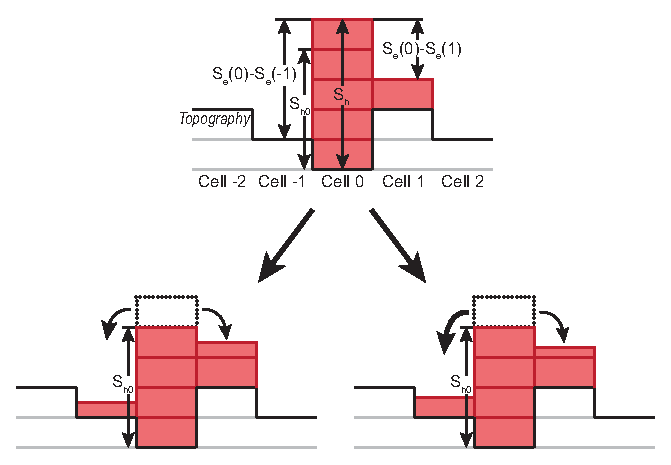
\includegraphics[width=0.5\linewidth]{figures/slope-proportional-example}
			\caption{A 2-D example of two transition functions. At timestep $t$ (top), Two cells are inundated with lava. The central cell (Cell 0) has 1 block of lava higher than the residual thickness, S$_{h0}$. In a slope-proportional sharing scheme, timestep $t+1$ will follow the path to the right; because Cell -1 has twice the relief as Cell 1, it receives twice as much of the residual lava (2/3 blocks vs. 1/3 to the right). In an equal-sharing scheme, the left path will be followed, and half the block will be added to both neighbor cells.}
			\label{fig_BernieSanders}
		\end{figure}
		
		\paragraph{Local slope-based spreading} In the LavaPL algorithm given by \citet{connor2012}, lava is apportioned from cells to their neighboring cells proportional to slope. To give a specific case, let a cell at location $c$ be the central cell, with a set of neighbor cells, X. The total relief between cell $c$ and its lower neighboring cells is 
		\begin{equation}
			\text{TR}(c) = \sum^{n\in \text{X}}(\text{S}_h(c)+\text{S}_e(c))-(\text{S}_h(n)+\text{S}_e(n))
			\label{eq_TR}
		\end{equation}
		where $\text{S}_h$ is the height or thickness of the lava in a cell, $\text{S}_e$ is the underlying elevation of the cell, and $n$ is a neighbor in X. The total lava to spread away from the central cell is the difference between thickness of lava (S$_h$) at $c$ the residual thickness (S$_{h0}$), unless the lava thickness is lower than the residual thickness, giving
		\begin{equation}
			\[ \text{Outbound}(c) =
			\begin{cases}
			\text{S}_h(c)-\text{S}_{h0}(c) & \quad \text{if } {S}_h(c)-\text{S}_{h0}(c) > 0\\
			0 & \quad \text{if } {S}_h(c)-\text{S}_{h0}(c) \le 0\\
			\end{cases}
			\]
			\label{eq_excess}
		\end{equation}
		
		In LavaPL, the excess flow, ``Outbound'', is delivered to neighbors $n$ based on the proportion of total relief, TR, found at each neighbor location (the right path of Figure \ref{fig_BernieSanders}). For each $n\in$X,
		\begin{equation}
			\text{Inbound}(n) = \text{Outbound}(c)\left(\frac{(\text{S}_h(c)+\text{S}_e(c))-(\text{S}_h(n)+\text{S}_e(n))}{\text{TR}}\right)
			\label{eq_propshare}
		\end{equation}
		This is the slope-proportional spreading equation. Another method would be ``slope-blind,'' and would spread lava to all lower neighbors equally following the equation
		\begin{equation}
			\text{Inbound}(n) = \left(\frac{\text{Outbound}(c)}{|\text{X}|}\right)
			\label{eq_equalshare}
		\end{equation}
		where $|\text{X}|$ is the size of the neighborhood, or the number of elements in the neighborhood. This is illustrated as the left path of Figure \ref{fig_BernieSanders}.
		
		\paragraph{Neighborhood size} The size of the neighborhood, X, in CA algorithms is commonly 4 or 8 in cardinal or ordinal directions. Here both have been implemented, which enables the benchmarks to test whether 8 spreading directions increases the performance of these tests. This is further described in the next section (\ref{sec_X}).

		\paragraph{Spreading inhibited by special relationships} Though the size of the neighborhood is set globally for all cells, neighbors are not guaranteed to receive lava from central cells. In all algorithms, for example, cells in the neighborhood that are higher than the central cell, including lava thicknesses, are excluded from the neighborhood set.
		
		\begin{figure}[!h]
			\centering
			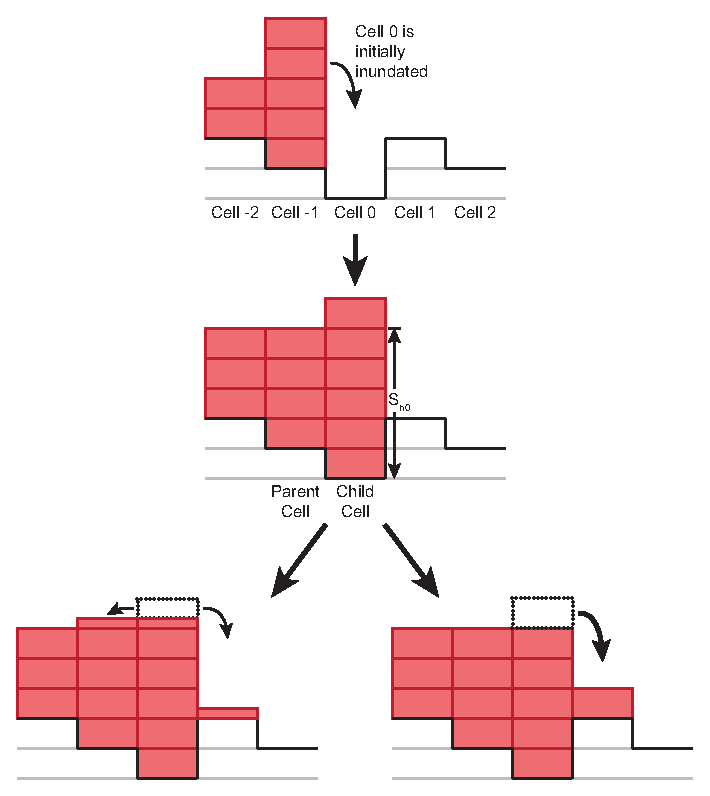
\includegraphics[width=0.5\linewidth]{figures/parent-child-example}
			\caption{Another 2-D example of different transition functions. In the first timestep (top), Cell -1 initially inundates Cell 0, creating the Parent-Child relationship shown in the next illustrated timestep (middle). If Parents cannot receive lava from Child cells, all residual lava in Cell 0 will flow to Cell 1, following the path to the right. If these relationships are ignored, as shown in the left path, Cell 0 will spread lava in both directions.}
			\label{fig_ParentTrap}
		\end{figure}
		
		Other neighbor elimination rules can also be implemented. One has been designed by \citet{connor2012}, where the cell that initially gives lava to another cell is forever eliminated from the receiving cell's neighborhood. This is done by creating a ``parent-child'' relationship for each activated cell in the flow. Simply put, child cells cannot give lava to their parent cells (right path in Figure \ref{fig_ParentTrap}). This transition function rule is tested against no parentage rules in competing MOLASSES algorithms (left path in Figure \ref{fig_ParentTrap}).
		
	\subsection{Cell Neighborhood, X}\label{sec_X}
	
	\begin{figure}[!h]
		\centering
		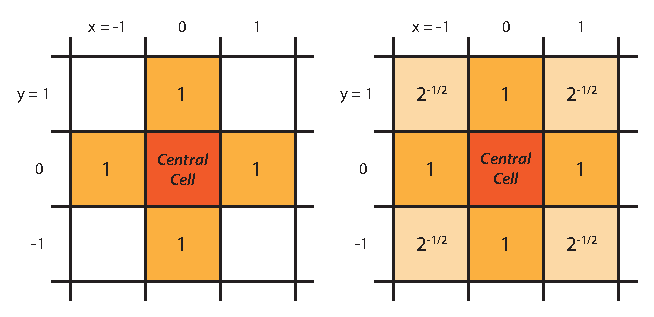
\includegraphics[width=0.5\linewidth]{figures/neighborhoods}
		\caption{Cellular Automata neighborhoods. To the left, in a 4-connected neighborhood, a central cell may influence or be influenced by cells in cardinal directions. To the right, in an 8-connected neighborhood, the zone of influence is expanded to include ordinal directions. Numbers in each cell are relative weights (determined by distance from the central cell), so diagonal neighbors are weighted less than orthogonal cells.}
		\label{fig_MrRogers}
	\end{figure}
	
		%NEIGHBOR_ID
		The final set in the CA is the cell neighborhood X and is defined by the \textbf{NEIGHBOR\_ID} module. This neighborhood is usually either 4-connected (von Neumann neighborhood) or 8-connected (Moore neighborhood) as illustrated in Figure \ref{fig_MrRogers}. Four-connected neighborhoods are defined as the row, column coordinates \{(0,1), (0,-1), (1,0), (-1,0)\}, where (0,0) is the location of a cell under evaluation, while the set elements might correspond to North, South, East, and West. Eight-connected neighbors include the ordinal directions, Northeast, Southeast, Northwest, and Southwest: \{(0,1), (0,-1), (1,0), (-1,0), (1,1), (-1,-1), (1,-1), (-1,-1)\}.
		
		NEIGHBOR\_ID is implemented within the DISTRIBUTE module to evaluate cells within X, and determine whether they are lower in elevation (including their lava) than the central cell. If one is lower, NEIGHBOR\_ID returns their relief, or the difference in elevation between the cell and the central cell, to the DISTRIBUTE module. Depending on whether parent-child relationships are recorded or ignored in the transition function, NEIGHBOR\_ID can follow one of two algorithms below.
		\begin{center}
		\begin{tabular}{l}
			\toprule
			\textbf{4-connected NEIGHBOR\_ID}\\
			\textbf{module}\\
			\midrule
			X = \{(0,1), (0,-1), (1,0), (-1,0)\}\\\\
			X' = \{\}\\
			$c$ = (0,0)\qquad (central cell location)\\
			\textbf{For} $n\in$ X\\
			~~\textbf{If}~$(\text{S}_h(c)+\text{S}_e(c))-(\text{S}_h(n)+\text{S}_e(n)) > 0$\\
			~~~~\textbf{Append}~$n$ to X'\\\\
			\textbf{Return}~X'\\
			\bottomrule
		\end{tabular}
		\begin{tabular}{l}
			\toprule
			\textbf{8-connected NEIGHBOR\_ID}\\
			\textbf{with Parent-Child Relationships}\\
			\midrule
			X = \{(0,1), (0,-1), (1,0), (-1,0), \\
			\qquad~(1,1), (-1,-1), (1,-1), (-1,-1)\}\\
			X' = \{\}\\
			$c$ = (0,0)\qquad (central cell location)\\
			\textbf{For} $n\in$ X\\
			~~\textbf{If}~$(\text{S}_h(c)+\text{S}_e(c))-(\text{S}_h(n)+\text{S}_e(n)) > 0$\\
			~~~~\textbf{If} $n$ is \textbf{not} Parent of $c$\\
			~~~~~~\textbf{Append}~$n$ to X'\\
			\textbf{Return}~X'\\
			\bottomrule
		\end{tabular}
		\end{center}


			
			
			
%%%%%%%%%%%%%%%%%%%%%%%%%%%%%%%%%%%%%%%%%%%%%%%%%%
%HIERARCHY
%%%%%%%%%%%%%%%%%%%%%%%%%%%%%%%%%%%%%%%%%%%%%%%%%%

	\section{Benchmarking Hierarchy}\label{sec:benchmark}
	
	The strategy implemented in this paper follows the advice of \citet{bayarri2007framework} for validating computer models, namely ``1) defining the problem; 2) establishing evaluation criteria; 3) designing experiments; 4) approximating computer model output; 5) analyzing the combination of field and computer run data.'' The sixth step in their validation process, feeding results back to revise models, has been done informally to determine how to alter spreading algorithms in future benchmarking attempts. Each level below presents a problem for a lava spreading algorithm to complete. These fundamental problems (e.g. replicating a Bingham flow) are evaluated using simple tests that demonstrate the problem. The relevant model output for each of these tests is a list of locations (i.e. a list of x and y coordinates) that have been inundated by lava. After verification (Level 0), the first validation level tests model results with other model results; the second level tests model output against expected analytical solutions; and the third level tests model output from field data.

	\begin{center}
		\begin{table}[h]
		\caption{Transition Algorithm Codes and Descriptions}
		\begin{tabular}{l c p{5cm} p{5cm}}
			\toprule
			Transition&Neighborhood&Parent-Child&Slope-proportional\\
			Function&&Relationships Preserved?&Sharing?\\
			\midrule
			\textbf{4/P/S} &4-directions & Yes, ``parents'' do not accept lava from ``children.'' & Yes, lower cells receive lava based on relative relief.\\
			\textbf{8/P/S} &8-directions & Yes & Yes\\
			\textbf{4/N/S} &4-directions & No, ``parents'' are not defined. & Yes\\
			\textbf{8/N/S} &8-directions & No  & Yes\\
			\textbf{4/P/E} &4-directions & Yes & No, all lower cells receive equal quantities of lava.\\
			\textbf{8/P/E} &8-directions & Yes & No\\
			\textbf{4/N/E} &4-directions & No  & No\\
			\textbf{8/N/E} &8-directions & No  & No\\
			
			\bottomrule
		\end{tabular}
		\label{tab_algorithmcodes}
		\end{table}
	\end{center}

\paragraph{Test Algorithms} Combining three variations of the Transition Function described in Section \ref{sec:MOLASSES}, I have created eight MOLASSES lava flow algorithms. Each variation has been made by modifying one module in the MOLASSES framework: The neighborhood is changed between 4- and 8- directions using the NEIGHBOR\_ID module, classifying one cell as a ``parent'' cell when a location is initially inundated is within the ACTIVATE module, and dividing lava amongst neighboring cells proportional to slope or equally is carried out in the DISTRIBUTE module. These eight algorithms will be referred to using three character codes, listed in Table \ref{tab_algorithmcodes}. For the algorithm used by LavaPL in \citet{connor2012}, the code would therefore be 4/P/S, as it spreads lava in 4-directions from a central cell, all inundated cells have designated parents to whom they cannot spread lava, and the quantity of lava to spread from a central cell is higher for lower neighboring cells.

	\subsection{Level 0: Conservation of Mass}
			Before the results of a lava flow simulation can be validated, it must be verified to at least prove that conservation of mass is preserved. A lava flow simulation will therefore not be tested against the following benchmark tests until this conservation of mass requirement is shown to be fulfilled.
			
			In MOLASSES, the code is verified within the DRIVER module, which manages each subordinate module. The erupted volume, $V_{in}$, is given as the total eruption volume specified by the user in the configuration file. If multiple source locations are given in this file, $V_{in}$ is the sum of total eruption volumes. $V_{in}$ is compared at the end of the module to the total volume of the flow, or $V_{out}$. The volume $V_{out}$ is calculated by summing the volume in all inundated grid cells. MOLASSES reports success if $V_{in}-V_{out} \le 10^{-8}$~m$^3$, which is the precision of a 64-bit double. If this test fails, MOLASSES reports failure and the excess volume found in the flow.
	
			\begin{center}
				\begin{tabular}{l}
					\toprule
					\textbf{MOLASSES Conservation of Mass Test}\\
					\midrule
					\textbf{If}~$|V_{in}-V_{out}| \le 10^{-8}$\\
					~~\textbf{Print}~\verb|SUCCESS: MASS CONSERVED|\\
					\textbf{Else}\\
					~~$excess = V_{out}-V_{in}$\\
					~~\textbf{Print}~\verb|ERROR: MASS NOT CONSERVED! Excess: |$excess$ \verb|m^3|\\
					\bottomrule
				\end{tabular}
			\end{center}

	\subsection{Level 1: Repeatability given meaningless parameter variation}
		Once the code has been verified to conserve mass, the flow can be validated. This first validation level tests that lava flow simulations are repeatable, regardless of changes in parameter space that should have no effect on the flow. Parameters that ideally should not effect lava flows include slope direction and elevation model resolution. For instance, a slope to the west and an identically dipping slope to the east should produce lava flows of equal length and shape (given identical flow attributes).
		
		\citet{miyamoto1997simulating} performed a simple validation test on two CA-like flow simulators \citep{ishihara1990numerical,miyamoto1997simulating} where a sloped DEM was rotated 45 degrees from ``south'' to ``southeast''. This benchmark was performed to demonstrate that the flow models had the same run-out length regardless of the arbitrary slope direction. Here, the DEM rotation scheme by \citet{miyamoto1997simulating} is adopted and expanded, so that a DEM of a simple slope is rotated 19 times at increments of 5$^{\circ}$. Flows are simulated on each of these slopes and the locations of inundated cells are output from the model.
		
		Three characteristics of the simulated flows are determined for each slope direction: flow length, orientation, and aspect ratio. Flow length is defined as the distance between the vent and the furthest inundated point from the vent. Flow orientation is defined as the direction that furthest point lies, with respect to North. Flow aspect ratio is the ratio of maximum flow width to flow length. Perfect success for this benchmark is when simulated flows, regardless of slope direction, 1) do not change in length, 2) have an orientation identical to the slope direction, and 3) do not change in aspect ratio. Failure is more subjective, but I will define failure as 1) more than 10\% variation in flow length depending on slope direction, 2) more than 5$^{\circ}$ offset between the slope and the flow orientation on average, or 3) more than 15\% variation in flow aspect ratio.
		
		\begin{figure}[h!]
			\centering
			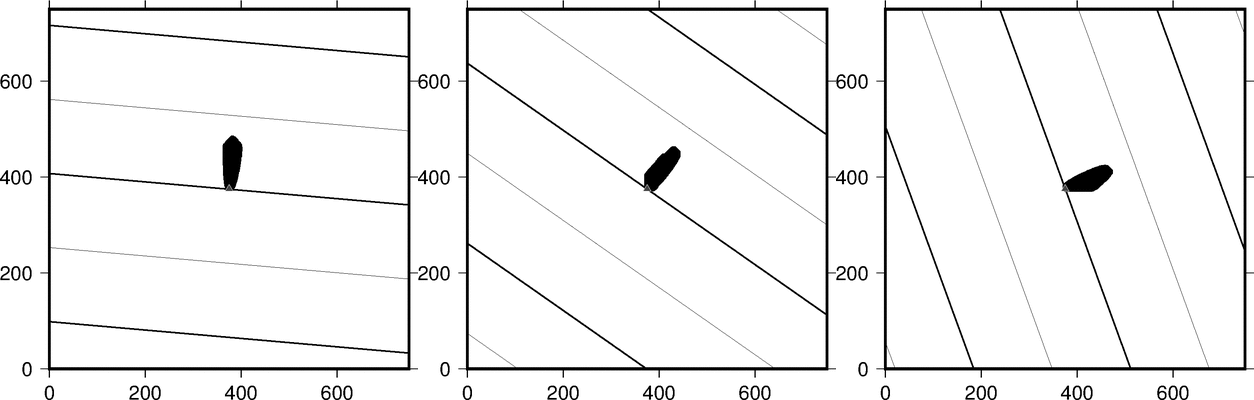
\includegraphics[width=\linewidth]{figures/lava_C_4N_slope}
			\caption{\textit{Rotating slope test for algorithm \textbf{4/P/S}. Slope dip is 18$^{\circ}$, with dip-directions 0N, 30N, and 80N from left to right. The flow length and aspect ratio are similar and the flow direction is in the slope direction, so even though the flow is oddly shaped, it passes Level 1 criteria.}}
			\label{fig:slope}
		\end{figure}
		
		\subsubsection{Benchmark Parameters} The underlying DEM for this benchmark has a simple 18$^{\circ}$ slope, dipping to the North. The DEM has a spatial resolution of 1~m. The source cell is placed at the center of the DEM, is given a total volume of 1000~m$^3$, and is given a pulse volume of 1~m$^3$. When the simulation is finished, model output is used to determing the three flow characteristics used in this benchmark (length, orientation, and aspect ratio). The DEM is rotated 5$^{\circ}$ clockwise and the process is repeated 19 times until the flow is simulated on an East-facing slope.
		
		
		
		\subsubsection{Results}

		For all eight flow algorithms, flow length, aspect ratio, and orientation were calculated 19 times, corresponding to the 19 dip directions sampled between 0$^{\circ}$N and 90$^{\circ}$N. Variance for length and aspect ratio were calculated as the ratio of their standard deviations to their means. For instance, if mean runout length for the 18 flows is 100~m and the standard deviation of the 18 lengths is 2~m, the runout length variance is 2\%. The mean direction error is also calculated for the set of flows from each algorithm. These are reported in the table below.

			\begin{center}
				\textbf{DEM Rotation Results}
				
				\begin{tabular}{l c c c}
					\toprule
					Transition&Run-out&Aspect Ratio&Mean Direction\\
					Function&Variance&Variance&Error\\
					\midrule
					4/P/S &2.7\%&6.7\%&1.2$^{\circ}$\\
					8/P/S &4.4&12.2&0.9\\
					4/N/S &9.6&19.7&1.3\\
					8/N/S &3.9&7.5&0.6\\
					4/P/E &21.6&38.6&14.2\\
					8/P/E &7.2&13.8&5.4\\
					4/N/E &21.6&38.7&14.1\\
					8/N/E &7.2&13.8&5.5\\
			
					\bottomrule
				\end{tabular}
			\end{center}

			While with an ideal spreading algorithm, variances and direction error would be 0 under a rotating slope, every spreading algorithm tested performed differently as DEM direction changed. Following from the above pass-fail standards, five of the eight algorithms can be rejected. Algorithms 4/P/E and 4/N/E have high run-out length variance. Algorithms 4/N/S, 4/P/E and 4/N/E have large aspect-ratio variance. Algorithms 4/P/E, 8/P/E, 4/N/E, and 8/N/E all systematically deviate from running downslope by $>5^{\circ}$ on average. This implies that algorithms which share lavas equally from central cells to all lower neighboring cells perform worse than algorithms which share lavas proportional to slope.
			
			For the eight different transition functions tested, runout length varied between 60-160~m. The flow algorithm with the least flow length variance was the 4-connected, parent-child, slope-proportional strategy implemented in LavaPL. Algorithms 4/P/S, 8/P/S, and 8/N/S cannot be rejected because of any of the three standards set in this benchmark.

	\subsection{Level 2: Replication of flow morphologies on simple physical surfaces}
	
	The second benchmarking level is the first step in validating lava flow algorithms against realistic flow expectations. Instead of parameter space being arbitrarily defined, which was the case in Level 1, the defined parameter space informs tests at this level as to what the model output should be. As lava flows on a large scale are well described as Bingham fluids, simulations can be tested against analytical solutions or experimental observations of these fluids in simple conditions. For instance, a lava flow on a perfectly flat surface might be expected to create a circular areal extent \citep{griffiths2000dynamics}.
	
			Here I measure flow algorithm performance on a flat surface from a single vent source location. To measure the extent to which the simulated flow replicates a circle, the inundated area is compared to the area of a circle which circumscribes the flow exactly. This can be described as
			\begin{equation}
				Fit = \frac{A_{flow}}{\pi d_{max}^2}
			\end{equation}
			where $d_{max}$ is the farthest extent of the simulated flow from the vent. A perfect match to a circle would result in a $Fit=1$. With the same maximum distance from the vent (i.e. the distance from the center to a vertex) a perfect square would cover 64\% of the area of a circle, ergo $Fit=0.64$. An octagon would have a fit of 0.90. We consider a model to successfully pass this test if it produces a flow of $Fit>0.90$, or if the flow approximates a circle better than an octagon. The model unambiguously fails this test if if produces a flow of $Fit<0.64$, where a square better describes a circle than a flow generated from the model.

			\begin{center}
				\textbf{Circular Flow Test}
				
				\begin{tabular}{l l}
					\toprule
					Fit = 1.0 & Best Possible Score; perfectly circular.\\
					Fit $>$ 0.90 & Success; better than an octagon. \\
					Fit $<$ 0.64 & Failure; worse than a square.\\
					\bottomrule
				\end{tabular}
			\end{center}
		
		\begin{figure}[!h]
		\centering
		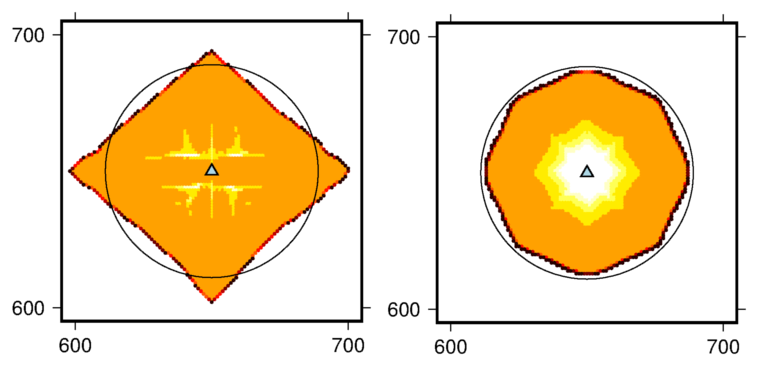
\includegraphics[width=\linewidth]{figures/pancake}
		\caption{Fitness scores of different shapes. From left to right: A circle has a perfect fit score of 1.00; an octagon has 0.90 times the area of a circumscribing circle; a square has a score of 0.64; Two flat surface tests for slope proportional spreading algorithms with parent rules. The flow second to the right is 4-connected (4/P/S) and has a score of 0.55, while the rightmost flow is 8-connected (8/P/S) with a score of 0.95. The 4/P/S flow fails the test as it scores worse than a square, while the 8/P/S flow passes the test as it scores better than an octagon.}
		\label{fig_pancake}
	\end{figure}
	
		\subsubsection{Benchmark Parameters} The DEM used in this benchmark is a horizontal plane (all grid locations have the same elevation) with a spatial resolution of 1~m. A single vent is located at the DEM center with a total volume of 1000~m$^3$, and a pulse volume of 1~m$^3$. When the simulation is finished, model output is used to find the inundated cell farthest from the vent ($d_{max}$). The total inundated area is divided by the area of a circle with radius $d_{max}$ to provide the Fit score.
		
		\subsubsection{Results}

		Five of the eight algorithms unambiguously passed the test of performing better than an octagon. Two algorithms unambiguously failed, one of which is the LavaPL algorithm (N/P/S) that outperfomed other models in the previous validation level. In this test 8-connected algorithms outperformed 4-connected algorithms.
		
		\begin{center}
			\textbf{Bingham Circle Results}\\
			\begin{tabular}{l c l}
				\toprule
				Algorithm&Circularity&\\
				\midrule
				4/P/S & 0.55 & Worse than a square.\\
				8/P/S & 0.95 & Better than an octagon.\\
				4/N/S & 0.55 & Worse than a square.\\
				8/N/S & 0.98 & Better than an octagon.\\
				4/P/E & 0.77 & Between a square and an octagon.\\
				8/P/E & 0.80 & Between a square and an octagon.\\
				4/N/E & 1.00 & Perfectly circular.\\
				8/N/E & 0.99 & Better than an octagon.\\
				
				\bottomrule
			\end{tabular}
		\end{center}
		
	\subsection{Level 3: Replication of real lava flows over complex topography}
		The recent availability of global or near-global topographic datasets, such as SRTM or ASTER GDEM has enabled the direct observation of the underlying surface of even more recent lava flows. The extents of lava flows such as the 2012-3 Tolbachik lava flow, in conjunction with available pre-eruption DEMs, is the final benchmarking test for lava flow algorithms. At this level, model inputs must reflect reality, which naturally makes parameter spaces used in applicable tests more complex than those used in previous levels. Ultimately, if a lava spreading algorithm succeeds at this level after performing well in previous levels, the algorithm is considered validated against field data.

		\subsubsection{2012-3 Tolbachik, Russia lava flows}\label{test:Real_Tolbachik}
			The goodness of fit between a simulated flow and a mapped lava flow can be simply measured by the Jaccard coefficient. This parameter is the ratio of the intersection area inundated by both the simulation and the real flows by the union area inundated by either. To illustrate, this test has been performed recently by Kubanek et al. (submitted) for the 2012-3 Tolbachik flow where a MOLASSES model configuration, explained later, produced a lava flow with a 59\% fit to the mapped flow. This result means that 59\% of the area inundated by either the simulated flow or the mapped flow, the union, was inundated by both the simulated and the mapped flows. Conversely, 41\% of the area was either modeled to have been inundated but wasn't or was modeled to be lava-free but actually was inundated by lava. These are generally known as false positives or false negatives, respectively.
			

			%Go on about how the Jaccard DEM is constructed maybe? or maybe this is results material.
			\begin{center}
				\begin{tabular}{l}
					\toprule
					\textbf{Test \ref{test:Real_Tolbachik} Algorithm}\\
					\midrule
					1.~$C_{real}$~:=~Locations of grid cells in Tolbachik DEM inundated by 2012-3 Flow.\\
					2.~Run \textbf{MOLASSES} over Tolbachik DEM\\
					3.~Define results:\\
						~\tabitem $C_{model}$~:=~Locations of cells, $C_i,...,C_N$, inundated by \textbf{MOLASSES} flow.\\
					4.~$Fit:=\cap_C/\cup_C$\\
						~\tabitem If $Fit\ge0.5$: Success\\
						~\tabitem If $Fit<0.5$: Failure\\
					\bottomrule
				\end{tabular}
			\end{center}
			
	\subsubsection{Results}
	
	Each transition function was tested over SRTM topography and a TanDEM-X DEM using values gathered from TanDEM-X analysis. Two vents were situated over the topography at UTM coordinates of the two active vents created in the 2012-3 Tolbachik eruption. The total combined volume output from these two vents were 0.38~cubic~km. The residual thickness of the flow is 7.8~m and the pulse volumes were defined as the product of the thickness and the spatial resolution of the underlying DEM. The Jaccard fit for each flow algorithm is listed below for both DEMs.
		\begin{figure}[!h]
			\centering
			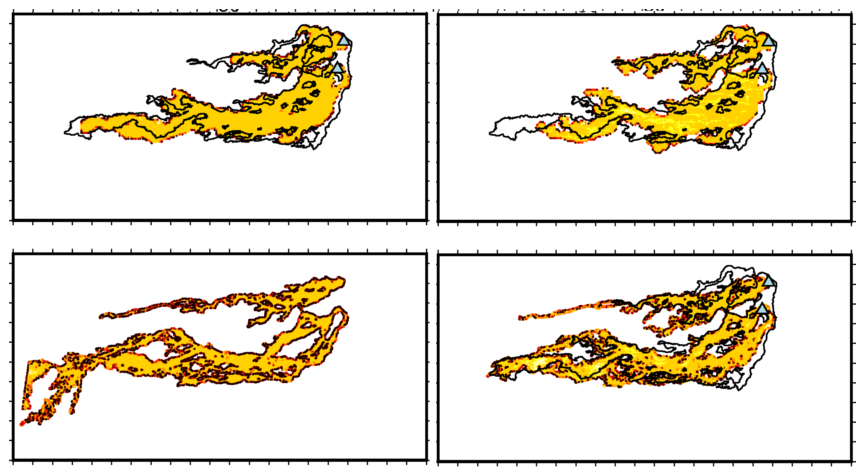
\includegraphics[width=0.7\linewidth]{figures/tolbachik}
			\caption{\textit{Two models run over two DEMs (SRTM, top; TanDEM-X, bottom) in the Tolbachik area. Left: An 8-connected, slope-proportional, no parent algorithm (8/N/S). Right: A 4-connected, equal spreading, no parent algorithm (4/N/E). Most spreading algorithms that had appropriate runout lengths in the SRTM test simulated very long flows over the TanDEM-X DEM. The mapped flow is plotted in black.}}
			\label{fig:tolbachik}
		\end{figure}
		
		\begin{center}
			\textbf{Tolbachik Flow Results}\\
			\begin{tabular}{l c c | c c}
				\toprule
				Transition&\multicolumn{2}{c}{\textbf{SRTM DEM}}&\multicolumn{2}{c}{\textbf{TanDEM-X DEM}}\\
				Function& Jaccard & Sensitivity& Jaccard & Sensitivity\\
				\midrule
				4/P/S & 56.7\%& 76.4\%& 53.0\%& 72.4\% \\
				8/P/S & 61.1  & 80.8  & 46.8  & 67.2   \\
				4/N/S & 57.2  & 77.5  & 44.0  & 64.0   \\
				8/N/S & 63.1  & 82.8  & 46.7  & 67.4   \\
				4/P/E & 51.2  & 71.5  & 54.2  & 73.4   \\
				8/P/E & 58.8  & 78.2  & 56.3  & 76.0   \\
				4/N/E & 54.5  & 74.5  & 55.7  & 73.7   \\
				8/N/E & 59.6  & 78.8  & 56.2  & 75.3   \\
				
				\bottomrule
			\end{tabular}
		\end{center}

		If success and failure are defined by having a fits of greater or less than 50\%, all models tested would pass for the SRTM DEM and about half would pass for the TanDEM-X DEM. All but one model performed worse on the TanDEM-X DEM.


%%%%%%%%%%%%%%%%%%%%%%%%%%%%%%%%%%%%%%%%%%%%%%%%
%BAYESIAN APPROACH
%%%%%%%%%%%%%%%%%%%%%%%%%%%%%%%%%%%%%%%%%%%%%%%%
%%%%%%%%%%%%%%%%%%%%%%%%%%%%%%%%%%%%%%%%%%%%%%%%
%%%%%%%%%%%%%%%%%%%%%%%%%%%%%%%%%%%%%%%%%%%%%%%%
\section{Bayesian Applications for Lava Flow Models}\label{sec:Bayesian}
	The final step \citet{bayarri2007framework} give for validating computer models is ``feeding [observations and results] back to revise the model.''
	
	The use of computer models to forecast hazards is a fundamentally Bayesian strategy: there is an initial concern due to hazards and computer models help us inform, constrain, and update this concern. Using Bayesian statistics can therefore be an improvement in testing lava flow models, over the two commonly used fitness tests, model sensitivity and the Jaccard index, because of their more direct application to informing perceived risk. 
	
	Three tools will be used in this section: A posterior probability, a ``negative'' posterior probability, and a Bayes factor. Bayes theorem connects a phenomenon $A$ to observations $B$ through the function
	\begin{equation}
		\text{Pr}(A|B)=\frac{\text{Pr}(B|A)\text{Pr}(A)}{\text{Pr}(B)}\label{eq_bayes}
	\end{equation}
	where $\text{Pr}(A)$ is the general probability of $A$ occuring, $\text{Pr}(B)$ is the probability of $B$ being observed, and $\text{Pr}(B|A)$ is the conditional probability of $B$ given the occurence of $A$. $\text{Pr}(B|A)$ is also known as model sensitivity and, in the specific case of lava flow modeling, can be stated as ``the percentage of the lava flow that the model correctly forecasted.''
	
	The left side of Equation \ref{eq_bayes}, $\text{Pr}(A|B)$, is the Posterior probability of $A$ and can be stated as ``the probability that lava will inundate a location if the model forecasted inundation at that location.'' A second posterior, which I call the negative posterior, is $\text{Pr}(\neg A|\neg B)$ and is the obverse of $\text{Pr}(A|B)$. This negative posterior relates not being inundated by lava at a given location to a safe outcome forecasted by a simulation and can be calculated by modifying Equation \ref{eq_bayes} and substituting $A$ for $Lava$ (the lava flow) and $B$ for $Sim$ (the simulation), resulting in the formula
	\begin{equation}
		\text{Pr}(\neg Lava|\neg Sim)=\frac{\text{Pr}(\neg Sim|\neg Lava)\text{Pr}(\neg Lava)}{\text{Pr}(\neg Sim)}
	\end{equation}
	where the $\neg$ symbol indicates the event or observation not happening, and $\text{Pr}(\neg Sim|\neg Lava)$ is model specificity.
	
	The negative posterior is important in hazard forecasting as it is in some sense a probability of safety. The more common posterior $\text{Pr}(A|B)$ (or $\text{Pr}(Lava|Sim)$) does not contain information about areas that the simulation does not inundate; while it can support the hypothesis that lava will hit a location given a simulated hit, it cannot estimate one's relative risk if the simulation forecasts a safe outcome. The negative posterior $\text{Pr}(\neg Lava|\neg Sim)$ does just this, and informs a user whether to rely on a safe outcome from a simulation. If, for example, the posterior probability $\text{Pr}(Lava|Sim)$ is high while the negative posterior probability $\text{Pr}(\neg Lava|\neg Sim)$ is low for a given lava flow simulator, areas that are evacuated due to the simulation outcome will be evacuated for good reason, but many areas will likely be inundated that were not evacuated due to the simulation outcome. This is why it is important to estimate and ultimately try to improve both posterior metrics.
	
	Bayes factors provide a tool to test the relative likelihood of a hypothesis against another. \citet{aspinall2003evidence} introduced this tool to volcano hazard forecasting by testing whether the onset of particular seismic events before the 1993 Galeras catastrophe was a significant indicator of the eruption or not. A Bayes Factor (BF) relating two models is given by \citet{jeffreys1998theory} as
	\begin{equation}
		\text{BF} = \frac{\text{Pr}(\text{Data}|\text{Model~1})}{\text{Pr}(\text{Data}|\text{Model~2})}
		\label{eq_BF}
	\end{equation}
	In the example of Galeras, the ``data'' are the seismic events, Model 1 is ``imminent explosion,'' and Model 2 is ``not imminent explosion'' \citep{aspinall2003evidence}. Below, I will apply this with the data being the probability of simulated inundation and the models ``lava inundation'' and ``not lava inundation.'' \citet{jeffreys1998theory} provided a log-scale interpretation to the value of BF in Equation \ref{eq_BF}, given in the table below.
	
	\begin{center}
			\textbf{Bayes Factor Interpretations (modified from \citet{aspinall2003evidence})}\\
			\begin{tabular}{l l}
				\toprule
				BF Value & Description\\
				\midrule
				$BF>10^2$ & Evidence for Model 1 is Decisive.\\
				$10^{1.5}<BF<10^2$ & Evidence for Model 1 is Very Strong.\\
				$10^{1}<BF<10^{1.5}$ & Evidence for Model 1 is Strong.\\
				$10^{0.5}<BF<10^{1}$ & Evidence for Model 1 is Substantial.\\
				$10^{0}<BF<10^{0.5}$ & Evidence for Model 1 is just worth a mention.\\\\
				$10^{-0.5}<BF<10^{0}$ & Evidence for Model 2 is just worth a mention.\\
				$10^{-1}<BF<10^{-0.5}$ & Evidence for Model 2 is Substantial.\\
				$10^{-1.5}<BF<10^{-1}$ & Evidence for Model 2 is Strong.\\
				$10^{-2}<BF<10^{-1.5}$ & Evidence for Model 2 is Very Strong.\\
				$BF<10^{-2}$ & Evidence for Model 2 is Decisive.\\
				\bottomrule
			\end{tabular}
		\end{center}
	
		In the same manner as the final validation level, the statistics discussed above will be calculated based on the areal extent of flows and simulations. The probability of the lava flow inundating an area $N$ can be given as
		\begin{equation}
			\text{Pr}(A)=\frac{|Lava|}{|N|}\label{eq_PA}
		\end{equation}
		where $|Lava|$ is the areal size of the flow (i.e. literally the number of DEM grid cells the lava inundates) and $|N|$ is the size of the area of interest, or the potential hazard area. The probability of the simulation is similarly found to be
		\begin{equation}
			\text{Pr}(Sim)=\frac{|Sim|}{|N|}.\label{eq_PB}
		\end{equation}
		By substituting these definitions and model sensitivity (Equation \ref{eq_sensitivity}, $|Lava \cap Sim|/|Lava|$) in Equation \ref{eq_bayes}, the posterior probability of lava flow inundation, given a simulation that forecasts inundation can be recast as
		\begin{align}
		\text{Pr}(Lava|Sim)&=\frac{\frac{|Lava\cap Sim|}{|Lava|}\frac{|Lava|}{|N|}}{\frac{|Sim|}{|N|}}~\text{,~or~simplified,}\label{eq_unsimplepost}\\
		&=\frac{|Lava\cap Sim|}{|Sim|}.\label{eq_simplepost}
		\end{align}
		where $|Lava\cap Sim|$ is the size of the intersection of the lava flow and simulated flow (again, the number of DEM grid cells). Note that this posterior probability is independent of the potential hazard area.
		
		The negative posterior can be stated in terms of the sizes of the lava flow and simulated flow as well.
		\begin{equation}
			\text{Pr}(\neg Lava|\neg Sim)=\frac{|\neg Lava\cap \neg Sim|}{|\neg Sim|}\label{eq_simplenegpost}
		\end{equation}
		Calculating the size or number of grid cells of $\neg Lava$ or $\neg Sim$ is fundamentally dependent on the potential hazard area, as $|\neg Lava|$ is defined as
		\begin{equation}
			|\neg Lava| = |N| - |Lava|.
		\end{equation}
		Because of this, we must define the size of the potential hazard area $N$ ($|N|$).	
	
	\paragraph{Potential Hazard Area} There are multiple strategies to estimating an \textit{a priori} hazard area. \citet{kauahikaua1995applications} for instance identified catchments or ``lava sheds'' in which a volcanic vent was erupting, and identified these lava sheds as the hazard area. \citet{kilburn2000lava} provided a theoretical maximum distance that a lava flow can travel given the mass flux of magma erupting at the vent location. A combination of these two would provide an objective hazard area defined as the area within the ``Kilburn distance'' that is topographically below the volcanic vent. The theoretical maximum distance, or hazard radius, given by \citet{kilburn2000lava} is
		\begin{equation}
		R_{max}=\sqrt{\frac{3\epsilon SQ}{\rho g\kappa}}
		\end{equation}
	where $\epsilon$ is an empirical value related to the amount of extension of lava crust allowed before it fails (10$^{-3}$), $S$ is the tensile strength of this crust (10$^7$~Pa), $\rho$ is the lava crust density (2200~kg~m$^{-3}$), $g$ is gravitational acceleration, $\kappa$ is the bulk thermal diffusivity ($4\times 10^{-7}$~m$^{2}$~s$^{-1}$) and $Q$ is the mean volumetric flow rate from the vent. From this, the hazard radius for the Tolbachik 2012-3 flow is calculated to be 39~km, given a magma flux of 440~m$^3$~s from the vent as was estimated early in the eruption \citep{belousov2015overview}. The total area within this radius that is also below the vent-plus-modal-flow-thickness elevation is 1,415~km$^2$. Note that the mapped flow area of 26~km$^2$ only covers 1.9\% of this defined hazard area (i.e. $\text{Pr}(Lava) = 0.019$).
	
	A second strategy would be to run many lava flow models from the known vent location(s) while varying input parameters. This would give a range of flows and the true flow might be completely contained within the region given by this range of simulations. Below, a Monte Carlo (MC) method will be used to simulate a large range of flows. If we define a potential hazard area as any location inundated by at least one simulated flow in this MC approach, the hazard area would be 72~km$^2$. As the mapped flow area from the Tolbachik eruption is 39\% of this area, it would be more practical to use this as the \textit{a priori} hazard area because it more reasonably reflects the potential inundation area. Both the Kilburn-Kauahikaua method and this MC method are illustrated in Figure \ref{fig_hazardarea}.
	
	\paragraph{Review of Validation Level 3} Instead of using model sensitivity and the Jaccard index as benchmarks for the various lava flow models, now the two posteriors will be used. The potential hazard area is defined as the distribution of MC simulations (72~km$^2$).
	
		\begin{center}
		\textbf{Traditional Fit Metrics and Bayesian Posterior Functions}\\
		\begin{tabular}{l c c c c}
			\toprule
			Transition&\multicolumn{4}{c}{\textbf{Results of simulations over SRTM DEM}}\\
			Function& Jaccard & Sensitivity & $\text{Pr}(Lava|Sim)$ & $\text{Pr}(\neg Lava|\neg Sim)$\\
			\midrule
			4/P/S & 56.7\%& 76.4\%& 70.4\%& 84.5\% \\
			8/P/S & 61.1  & 80.8  & 73.2  & 87.3   \\
			4/N/S & 57.2  & 77.5  & 70.3  & 85.1   \\
			8/N/S & 63.1  & 82.8  & 74.4  & 88.5   \\
			4/P/E & 51.2  & 71.5  & 66.0  & 81.4   \\
			8/P/E & 58.8  & 78.2  & 72.0  & 85.7   \\
			4/N/E & 54.5  & 74.5  & 68.7  & 83.3   \\
			8/N/E & 59.6  & 78.8  & 72.8  & 86.2   \\
			
			\bottomrule
		\end{tabular}
	\end{center}
	
	For the rest of this section, the preferred model, 8/N/S (the 8-connected, no parent-child relationships, with slope-proportional spreading) algorithm will be used. By applying this model to the Tolbachik lava flows, Bayesian methods will be used to improve the ``Pulse Volume'' parameter and will later be used to constrain model uncertainty at Tolbachik.
	
	\subsection{Improving model performance on one model parameter}
	
	
	\subsection{Incorporating Model Uncertainty with a Monte Carlo method}
		Model uncertainty is a result of input parameter uncertainty, such as uncertainty in the underlying DEM. This can be distinguished from model error, which might be defined as the difference between the true lava flow and a simulation carried out with perfect input parameters, and is created by the inherent deviations between a computer model and real life processes. Because there is parameter uncertainty, it is essential to quantify the range of model solutions given the likely range of each parameter.
		
		In this example, elevation uncertainty will be examined. Elevation uncertainty is an element in the MOLASSES module \textbf{INITFLOW}, where each grid cell elevation can be defined randomly before the lava flow simulation begins. The user can add an elevation uncertainty, in meters, to the configuration file. If this value is provided, each grid cell will receive a new elevation value randomly selected from a normal distribution whose mean is the DEM elevation and the standard deviation is the uncertainty value.
		
		The Monte Carlo method runs MOLASSES 100,000 times over a 75-m SRTM DEM. Vertical uncertainty of this data is estimated by \citet{rodriguez2006global} for Eurasia to be 6.2~m at a 90\% confidence level and is shown to be randomly distributed. With this result, elevation uncertainty in the MOLASSES model is given a value of $1\sigma=3$~m. Other input parameters remain unchanged from the benchmark exercise above; MOLASSES flow parameters for the Monte Carlo model are listed below. The combined 100,000 simulations are mapped in Figure \ref{fig:MC_map} where flow color indicates the number of flows that impacted each location.
		
		\begin{center}
			\textbf{Monte Carlo MOLASSES Flow Parameters}\\
			\begin{tabular}{l l}
				\toprule
				Elevation Model & 75-m SRTM\\
				Elevation Uncertainty, $1\sigma$ & 3~m\\
				Residual Thickness & 7.8~m\\
				Pulse Volumes & 44200 m$^3$\\
				\midrule
				Vent$_N$ Easting & 582800~m (UTM Zone 57)\\
				Vent$_N$ Northing & 6182100~m\\
				Vent$_N$ Total Volume & 4.63$\cdot10^7$~m$^3$\\
				\midrule
				Vent$_S$ Easting & 582475~m\\
				Vent$_S$ Northing & 6180700~m\\
				Vent$_S$ Total Volume & 1.737$\cdot10^8$~m$^3$\\
				\bottomrule
			\end{tabular}
		\end{center}

		%Map of the MC flows
		\begin{figure}
			\centering
			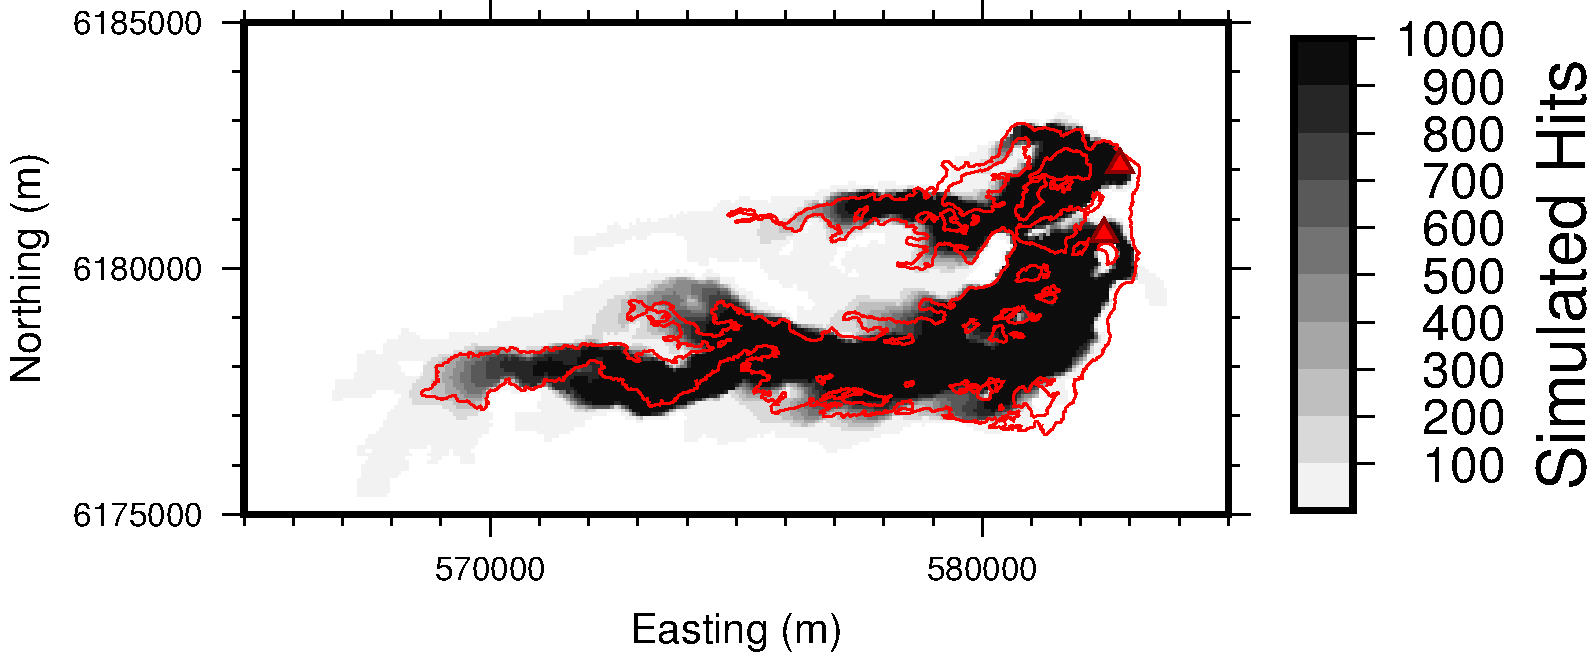
\includegraphics[width=0.7\linewidth]{figures/MC_map}
			\caption{Cumulative distribution of 1,000 simulated lava flows over SRTM topography with 3~m elevation uncertainty. The red outline is the mapped flow extent of the 2012-3 Tolbachik flow. The flow source vents are mapped as red triangles.}
			\label{fig:MC_map}
		\end{figure}
				
		\subsubsection{Bayesian distribution of MC results}
				Again, the reliability of a model can be better understood by showing the distribution of model performance given model uncertainty, as opposed to treating model parameters, and thus model output, as completely certain. Figure \ref{fig:MC_dist} shows the distribution of the posterior and the negative posterior.  
		
		\paragraph{Discuss distribution compared to the} lines drawn for the original simulation (0 m elev uncert).


		%Graph of the performances
		\begin{figure}
			\centering
			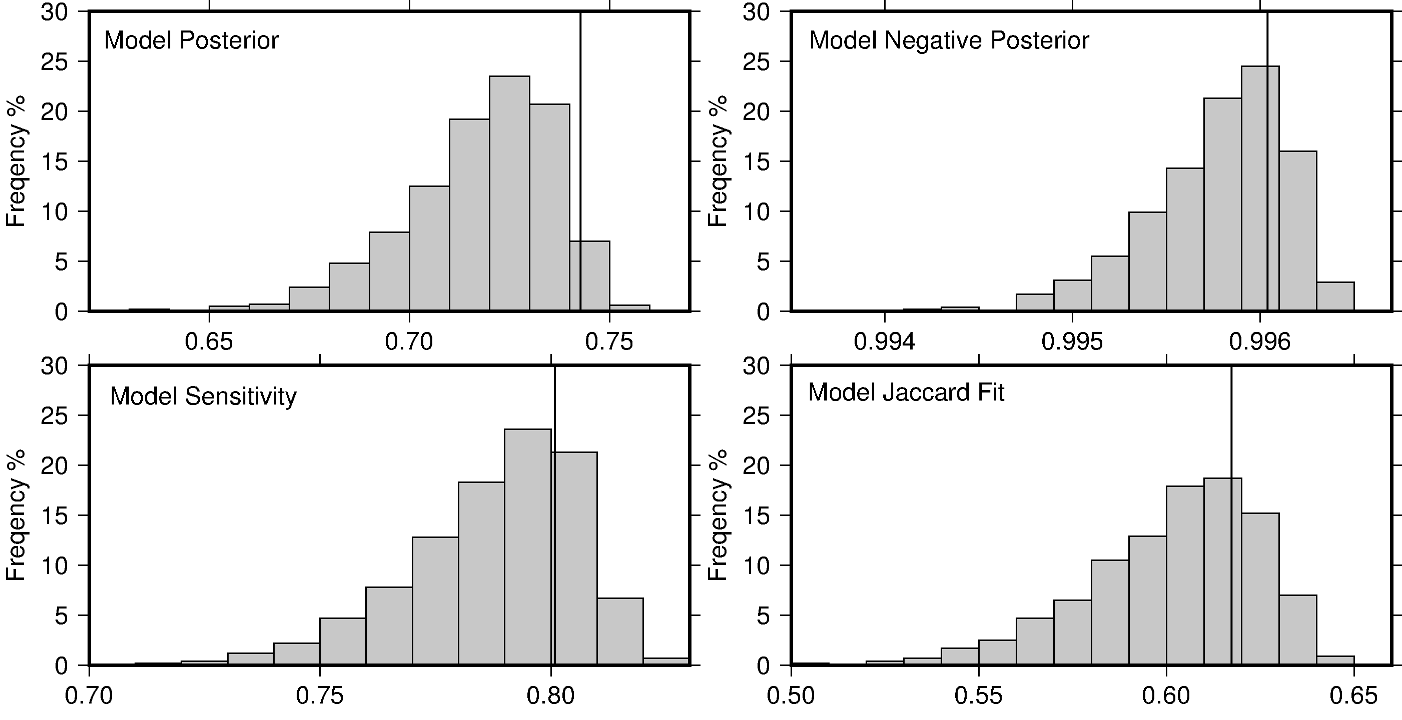
\includegraphics[width=0.7\linewidth]{figures/bayes_graphs}
			\caption{Distributions of fitness statistics between the 2012-3 Tolbachik Lava Flows and 1,000 simulated lava flows over SRTM topography with 3~m standard elevation uncertainty. Vertical lines are the fitness of a simulated lava flow run over SRTM data assuming 0~m elevation uncertainty. The better than average fit for this simulation might suggest that topography is locally known better than 3~m.}
			\label{fig:MC_dist}
		\end{figure}

		\subsubsection{Estimating inundation risk from the simulated frequency of inundation}
		
%%%%%%%%%%%%%%%%%%%%%%%%%%%%%%%%%55
%%%%%%%%%%%%%%%%OLD BAYES SECTION%%%%%%%%%%%%%%%%%
%%%%%%%%%%%%%%%%%%%%%%%%%%%%%%%%%55
\section{Old Bayes Section}

	\subsection{Improving Model Performance}\label{sec:lava_app}
		A primary way that hazard forecasting models have been validated in the past has been asking the question ``What percentage of the hazard phenomenon did the model correctly forecast?'' This is essentially asking for the model sensitivity. A person at risk of loss due to the hazard might instead want to know ``If the model forecasts loss for me, what is the likelihood that loss will actually occur?'' This is the posterior probability, $P(A|B)$ discussed above.

		Applied to lava flows and lava flow models, the population $N$ can be considered to be locations that might possibly be inundated with lava, given an eruption. The phenomenon $A$, in this case eventual inundation by lava, occurs or does not occur for each location and $P(A)$ is the probability of inundation within $N$. The test $B$ for each element in $N$ is an algorithm which models lava inundation and $P(B)$ is the probability of the flow simulation forecasting inundation within $N$. Equation \ref{eq_bayes} can be altered to:
		\begin{equation}
		P(Lava|Sim)=\frac{P(Sim|Lava)P(Lava)}{P(Sim)}\label{eq_lavabayes}
		\end{equation}
		where $Lava$ is the real phenomenon of lava inundation and $Sim$ is the model prediction of inundation, at any given location within the assigned hazard area of interest.

		Analysis performed on the 2012-3 Tolbachik flow presents an opportunity to validate lava flow models in a Bayesian framework: pre-eruptive DEMs exist at multiple spatial resolutions (e.g.~75~m SRTM and 15~m TanDEM-X), the locations of flow inundation have been mapped, and flow parameters have been estimated or measured (e.g. magma flux at the source vents, locations of source vents, flow thickness, flow volume). Lava flow models can be run using the flow parameters and pre-eruptive DEMs as input parameters, giving the subpopulation $Sim$. The mapped lava flow provides the subpopulation $Lava$. Comparing $Sim$ for different algorithms directly with $Lava$ can then quantify the valditiy of flow algorithms in a Bayesian sense.

		\paragraph{Model Execution} To populate $Sim$, I have run the MOLASSES lava flow code using TanDEM-X derived parameters, listed below:
		\begin{center}
			\textbf{MOLASSES Flow Parameters}\\
			\begin{tabular}{l l}
				\toprule
				Elevation Model & 15-m bistatic TanDEM-X, 11 Nov 2015\\
				Modal Thickness & 7.8~m\\
				Pulse Volumes & 16 equally separated volumes, [1755,14917] m$^3$\\
				\midrule
				Vent$_N$ Easting & 582800~m (UTM Zone 57)\\
				Vent$_N$ Northing & 6182100~m\\
				Vent$_N$ Total Volume & 4.63$\cdot10^7$~m$^3$\\
				\midrule
				Vent$_S$ Easting & 582475~m\\
				Vent$_S$ Northing & 6180700~m\\
				Vent$_S$ Total Volume & 1.737$\cdot10^8$~m$^3$\\
				\bottomrule
			\end{tabular}
		\end{center}
		All variables are fixed except the ``Pulse Volume'' parameter, which is the amount of lava delivered to source cells in the Cellular Automata grid of MOLASSES.

		Model output is compared to a list of x,y locations in the Tolbachik area that have been inundated or not. This location list is stored in a raster with the same projection and extent as the elevation model used in MOLASSES. ASCII locations output by MOLASSES are also listed in the same projection within the same extent as the elevation model. This enables direct comparison between the Model information (i.e. $Sim$) and the mapped lava flow (i.e. $Lava$). True Positives, False Positives, and False Negatives are reported as cell counts (number of grid locations where $Lava$ and $Sim$ agree or not). Three examples of these simulations are mapped in Figure \ref{fig:pulse_map}.

		\begin{figure}
		\centering
		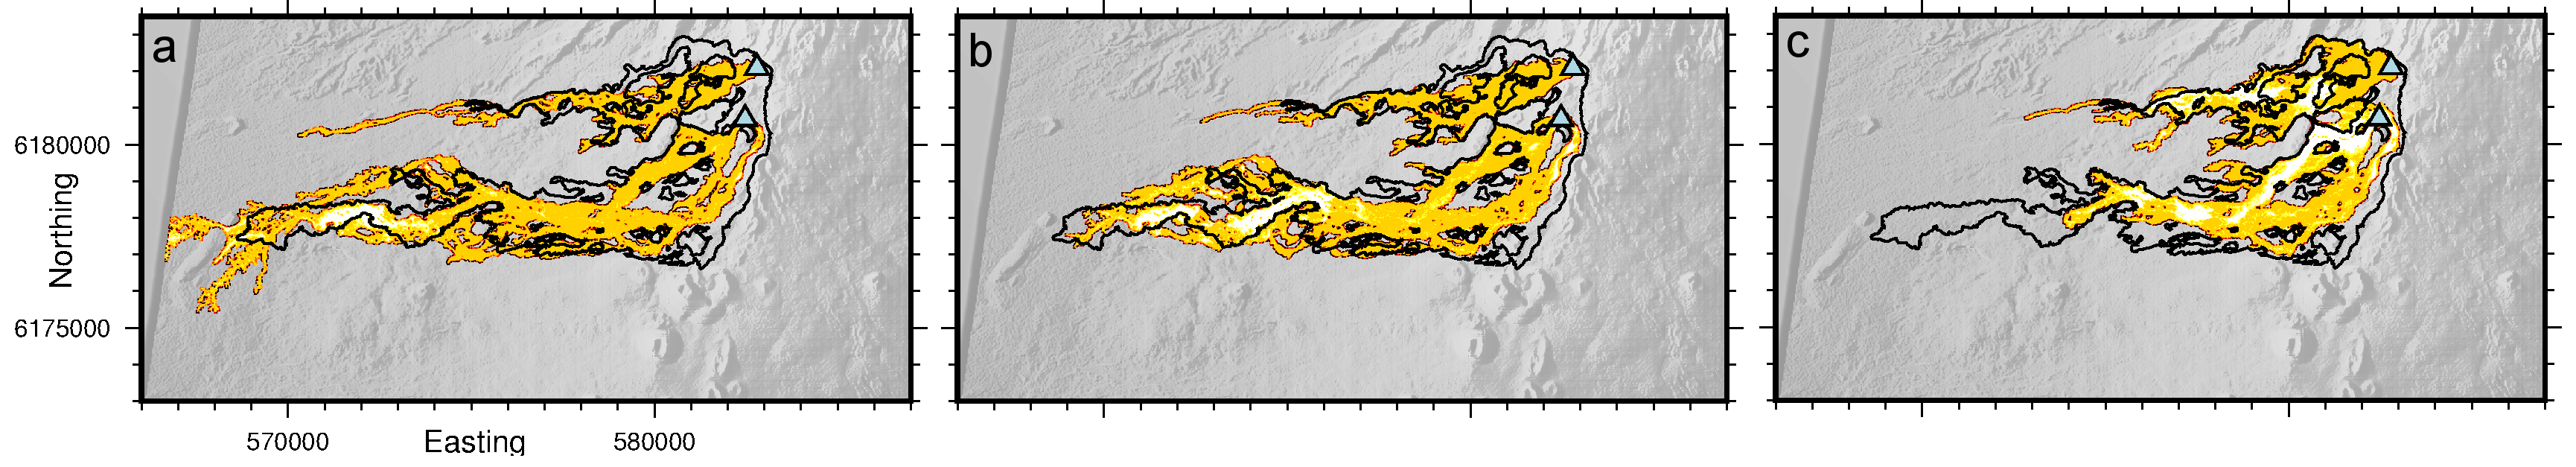
\includegraphics[width=\linewidth]{figures/3flows_h}
		\caption{MOLASSES Simulations of the 2012-3 Tolbachik Lava Flows. Vents are shown as blue triangles and the mapped flow is outlined in black. a) Pulse Volume = 1755 m$^3$, the simulation far exceeds the true runout distance; b) Pulse Volume = 4387 m$^3$, this simulation performs best under the negative posterior $P(\neg Lava|\neg Sim)$ test; c) Pulse Volume = 14040 m$^3$, this simulation performs best under the posterior $P(Lava|Sim)$ test, but does not have a runout length similar to the mapped flow.}
		\label{fig:pulse_map}
		\end{figure}

		\subsubsection{$P(Sim|Lava)$ (model sensitivity): Lava destroyed my home, but did the simulation predict it?}

		Model sensitivity is the percentage of the true phenomenon $Lava$ that the test $Sim$ accurately predicted. A model sensitivity of 0\% would indicate that between $Lava$ and $Sim$ there were no true positives. Mathematically, the size of the union, $|Lava\cap Sim|$ is 0. A model sensitivity of 100\% would indicate that $|Lava\cap Sim|$ is the same size as $Lava$, or $|Lava\cap Sim|=|Lava|$. If model sensitivity is perfect, there are no false negatives, though there might be false positives.

		\subsubsection{$P(Lava|Sim)$: If the simulation predicts lava inundation for a given location, what is the actual chance of lava inundation at the location?}

		The posterior statistical measure is the fundamental tool of Bayesian statistics, and quantifying it enables an update of belief in risk of lava inundation. A perfect posterior value would mean that if the model simulates lava inundating a location, lava will certainly inundate that location. The posterior is calculated for simulated lava flows of different Pulse Volumes and is graphed in Figure \ref{fig_lavaGsim}. From this, it can be seen that the highest pulse volumes, which coincidentally form the shortest flow simulations, perform best with this test, with the best fit having a pulse volume of 14040~m$^3$ per algorithm loop (Figure \ref{fig:pulse_map},c). A local maximum does exist in the low pulse volumes at 4387~m$^3$ per loop.


		\begin{figure}[h!]
			\centering
			\begin{gnuplot}[terminal=latex, terminaloptions=rotate]
				unset key
				set size 0.7,0.7
				set format xy "$%g$"
				set xlabel "Pulse Volume (m$^3$)" rotate by 90
				set ylabel "$P(Lava|Sim)$"
				set ytics 0.05
				set xtics 4000
				plot "results_bayes.dat" using 1:2 with linespoints lt 4 pt 7
			\end{gnuplot}
			\caption{Posterior $P(Lava|Sim)$ for MOLASSES flows with differing Pulse Volumes.}
			\label{fig_lavaGsim}
		\end{figure}

		%Talk specifically about the math
		%Provide examples as figures.

		\paragraph{Hazard Response Implications} The higher $P(Lava|Sim)$ is for a lava spreading algorithm, the higher certainty there is that if the simulation predicts inundation, inundation will occur. Algorithms known to have high $P(Lava|Sim)$ values should influence more people to evacuate an area, if the area is predicted by those algorithms to be hit by lava. If $P(Lava|Sim)$ is low, then it is more likely that evacuating all locations simulated to be affected would be a waste of resources.

		\subsubsection{$P(\neg Lava|\neg Sim)$: If the simulation predicts my safety, how safe am I really?}\label{sec_negpost}

		The weakness of the posterior statistic explored so far ($P(Lava|Sim)$), is that it does not measure fit of the negative results of the simulation. If the simulation does not inundate a location, this posterior does not enable the ``belief of safety,'' $P(\neg Lava)$, to be updated. Therefore I propose to use a second posterior, which I will call the \textit{negative posterior}.

		The negative posterior $P(\neg Lava|\neg Sim)$, or the probability of safety given simulated safety, is essentially the percentage of non-inundated area in the simulation that is also not inundated in real life. This can be found by defining this posterior using Bayes' Theorem similar to Equation \ref{eq_lavabayes}:
		\begin{equation}
		P(\neg Lava|\neg Sim)=\frac{P(\neg Sim|\neg Lava)P(\neg Lava)}{P(\neg Sim)}
		\end{equation}
		A perfect negative posterior would indicate that, if a model does not simulate a hit for a location, lava will certainly not inundate that location. While the posterior $P(Lava|Sim)$ is essentially population size blind, and does not rely on the number of true negatives (Equations \ref{eq_unsimplepost} and \ref{eq_simplepost}), this posterior does rely on true negatives. Thus, the size of the population, here referred to as the Potential Hazard Area, must be estimated \textit{a priori}.

		\paragraph{Results}


		\begin{figure}[h!]
			\centering
			\begin{gnuplot}[terminal=latex, terminaloptions=rotate]
				unset key
				set size 0.7,0.7
				set format xy "$%g$"
				set xlabel "Pulse Volume (m$^3$)" rotate by 90
				set ylabel "$P($not $Lava|$not $Sim)$"
				set ytics 0.01
				set xtics 4000
				plot "results_bayes.dat" using 1:3 with linespoints lt 4 pt 7
			\end{gnuplot}
			\caption{Negative posterior $P(\neg Lava|\neg Sim)$ for MOLASSES flows with differing Pulse Volumes.}
			\label{fig_neglavaGsim}
		\end{figure}

		The negative posteriors of simulations with different pulse values are shown in Figure \ref{fig_neglavaGsim}. Unlike the previous posterior analyzed, the best performing flows have smaller pulse volumes and the best performing volume is 4387~m$^3$ per model pulse loop (Figure \ref{fig:pulse_map},b). These results, however, show very high performance for all models, where $>$99.2\% of the area not hit by the lava flow in the potential hazard area is also not hit in all simulations. This is due to the enormous relative size of the hazard area and will be discussed later. Also of note, due to the large potential hazard area, this posterior has a very strong correlation with Model Sensitivity (Figure \ref{fig_sensitivity}). The correlation is not a coincidence. These two metrics will always have a high linear agreement given a very large abundance of true negatives. This fact is explained in an Appendix following this report.

		\paragraph{Hazard Response Implications} The higher $P(\neg Lava|\neg Sim)$ is for a lava spreading algorithm, simulated safety (i.e. the similation does not predict inundation) at a given location more certainly predicts real safety at that location. This is the obverse of the previously discussed posterior metric, which relates simulated damage to actual damage. Algorithms known to have high $P(\neg Lava|\neg Sim)$ values should influence fewer people to evacuate an area that is predicted by those algorithms to be safe. If $P(\neg Lava|\neg Sim)$ is low however, it is more likely that necessary evacuations would not occur, resulting in greater loss of infrastructure or even life.

	\subsection{Incorporating Model Uncertainty with Monte Carlo}\label{sec:lava_MC}

\subsubsection{Model fit at different simulated inundation probabilities}
By creating a cumulative map of lava flow simulations in the Monte Carlo (Figure \ref{fig:MC_map}), $P(Sim)$ may be estimated for every location as opposed to for the entire hazard area.


\begin{figure}[!h]
		\centering
		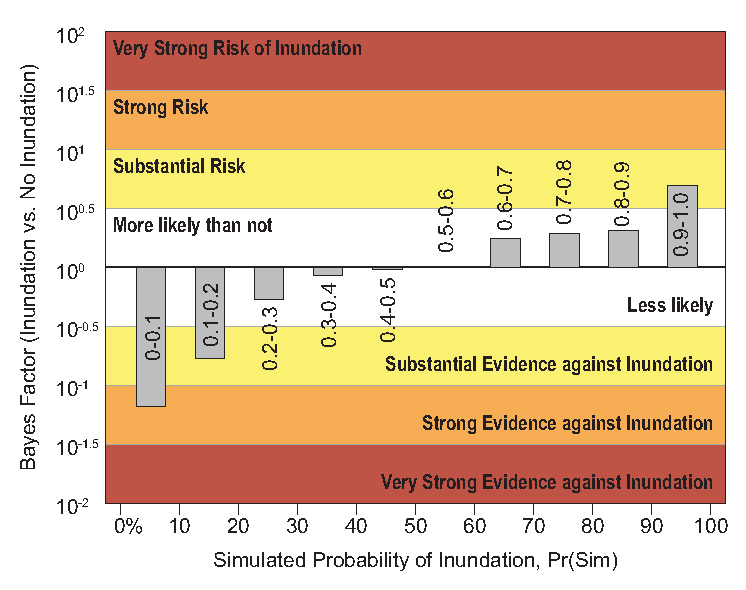
\includegraphics[width=0.7\linewidth]{figures/LR_bayes}
		\caption{Whether you should believe the MC or not}
		\label{fig_bayesfactor}
	\end{figure}

I have selected different subsets of the cumulative distribution of lava flows to evaluate using both posterior statistics, based on how many simulations hit given locations. Subsets are defined as all locations where at least a given percentage of simulated flows hit (e.g. the set of locations hit by more than 60\% of simulations, the set of locations hit by all simulations). The model fit between these subsets and the Tolbachik Flows are charted in Figure \ref{fig:MC_cum}. Points in this figure represent the probability of lava flow inundation at locations within each of these subsets. For example, 88\% of locations hit by every simulation are mapped as inundated; 75\% of locations hit by at least half of all simulations were inundated by lava; and 44\% of locations hit by at least one simulation were inundated by lava. The negative posterior is also charted in the same way: locations within the hazard area that were never hit by simulations were 99.9\% likely to remain uninundated; locations hit by fewer than half of all simulations were 99.6\% likely to not be inundated by lava; while only 98.7\% of areas remained uninundated when only locations hit by 100\% of simulations were removed.

By using this Monte Carlo method to incorporate uncertainty for an advancing lava flow, each location is assigned a probability of inundation by simulations. As the simulation is not perfect, this probability is not the same as the probability of actual inundation by lava (which is the whole reason for this report, after all). If a location is found to have a 20\% chance of inundation among simulated flows, is this similar to the probability of actual inundation? In Figure \ref{fig:MC_split} the posterior $P(Flow|Sim)$ is calculated for all locations hit by given percentages of simulations. Areas hit by $<$5\% of simulated flows all have a roughly 5\% chance of being inundated by the real flow. A positive correlation between this posterior and probability of simulation does exist in this view. The correlation appears to roll off as $P(Sim)$ approaches 65\%, as the limit of the model is reached.



%%%%%%%%%%%%%%%%%%%%%%%%%%%%%%%%%%%%%%%%%%%%%%%%
%DISCUSSION
%%%%%%%%%%%%%%%%%%%%%%%%%%%%%%%%%%%%%%%%%%%%%%%%
%%%%%%%%%%%%%%%%%%%%%%%%%%%%%%%%%%%%%%%%%%%%%%%%
%%%%%%%%%%%%%%%%%%%%%%%%%%%%%%%%%%%%%%%%%%%%%%%%

\section{Discussion}\label{sec:discussion}
	\subsection{Validation levels 1 and 2}
	A valid model can be determined by elimination. Spreading algorithms that are not slope-proportional spreading methods can be eliminated in the Level 1 test. Of the four remaining algorithms, only 8-connected transition functions succeed in Level 2. Luckily, both of these 8-connected, slope-proportional spreading funtions also perform best in replicating the Tolbachik flows over SRTM. However, they do not pass the 50\% fit test over TanDEM-X.
	
	One reason why most flows do worse over the TanDEM-X DEM could be due to the Pulse Volume used. While this pulse volume is convenient, as it is defined by parameters known \textit{a priori}, it might be essential to test a range of pulse parameters to refine this parameter and find the best possible fit of flows over TanDEM-X data. This is the sixth and final step of the validation guide given by \citet{bayarri2007framework}.
	
	Overall, in all tests 8-connected models outperfom 4-connected models. While equal sharing algorithms outperfom slope-proportional sharing on a flat slope, they fail on a rotating DEM and perform about the same on real topography. There does not seem to be an unambiguously better choice between using parent-child relationships or not. If future tests continue to show similar performance between models with and without parentage, other reasons can be used to choose a model, such as computer run-time. Currently, the perferred model is one that spreads in 8 directions without parentage rules that delivers lava in a slope-proportional fashion.
	
	The strength of the MOLASSES code is that new algorithms, such as those used in the SCIARA model, can be implemented relatively quickly and run through the Benchmarking tests, which are written in Python. Combinations of implementation strategies can also be created on the fly by adjusting the makefile of the MOLASSES code instead of the code itself.

	\subsection{Validation level 3: Bayesian applications for real lava flows}
		Validation of lava flow models is important as a method of increasing the value of models to forecast lava flow processes, thereby decreasing preventable loss. Preventable loss can either be loss of property due to lava or expenditure of resources on a lava flow that never comes. Because loss of property is necessarily more valuable than a loss of resources to protect that property (since, if the resources to protect the property were more valuable, it would not make sense to use those resources), the posterior probability $P(\neg Lava|\neg Sim)$ is more important that the posterior probability $P(Lava|Sim)$. However, because $P(\neg Lava|\neg Sim)$ is dependent on the population size (i.e. the potential hazard area), it is harder to quantify.

		\subsubsection{Using Bayesian statistics to compare models}

		In the pulse volume exercise, both the posterior and the negative posterior metrics were calculated for a number of simulations with differing pulse volumes. One pulse volume, 14040~m$^3$ per loop, performed best using the posterior statistic (Figure \ref{fig_lavaGsim}) and another, 4387~m$^3$ per loop, performed best using the negative posterior (Figure \ref{fig_neglavaGsim}). An optimal pulse volume can be identified if these metrics are given weight and compared. Because it is likely more important to have fewer false negatives (where destruction is unexpected) than false positives (where evacuation occurs but is not eventually needed), one might weight the negative posterior more importantly than the other posterior.

		To score simulations by combining the posteriors, I have normalized both posteriors so the worst scoring flow has a value of 0 and the best has a score of 1. I then took a weighted average of the normalized posteriors assuming the negative posterior is 10, 5, 2, and 1 times as important as the other posterior. These are graphed on the right of Figure \ref{fig:jaccard_combined}. Luckily, regardless of the weighting, the same pulse volume is always ranked highest (4387~m$^3$ per loop).

		It is interesting to note that the Jaccard Fit for these simulations (plotted on the left side of Figure \ref{fig:jaccard_combined}) is similar in shape to the weighted scores. The Jaccard fit is most similar to the combined scores where the posterior and negative posterior are given equal weight. In this case the correlation between the combined scores and the Jaccard fits have an r$^2$ value of 0.98.

		%%%%NOTES%%%%
		%The Jaccard model appears to be related to both posterior functions
		%Changing Population size (Improvement in neg Post and Improvement in learning)
		%Weighted average

		\begin{figure}[h!]
			\centering
			\begin{gnuplot}[terminal=latex, terminaloptions=rotate]
				unset key
				set size 0.7,0.7
				set format xy "$%g$"
				set xlabel "Pulse Volume (m$^3$)" rotate by 90
				set ylabel "Model Score"
				set ytics 0.02
				set xtics 4000
				plot "results_bayes.dat" using 1:7 with points pt 1, "results_bayes.dat" using 1:5 with points pt 7, "results_bayes.dat" using 1:6 with points pt 3, "results_bayes.dat" using 1:4 with points pt 6
			\end{gnuplot}
			\caption{Weighted averages of $\text{Pr}(Lava|Sim)$ and $\text{Pr}(\neg Lava|\neg Sim)$ for different pulse volumes. Hollow circles, negative posterior ($\text{Pr}(Lava|Sim)$) is given 10$\times$ the weight of the posterior ($\text{Pr}(\neg Lava|\neg Sim)$); solid circles, 5$\times$ weight; asterisks, 2$\times$ weight; plusses, equal weight between posteriors. The ``best'' Pulse Volume is 4387 (m$^3$) for all weight ratios except when both posterior values are weighted equally.}
			\label{fig_weightedposteriors}
		\end{figure}
		
		\subsubsection{Bayesian Conclusions}
			Regardless of how a lava flow model is chosen, its value in forecasting lava flow hazards can be quantified using Bayesian statistics. Whether the model is bad or good, if it can be compared against a real life lava flow such as the 2012-3 Tolbachik flow, the two posteriors discussed in this paper can be calculated.

			By calculating $P(\neg Lava|\neg Sim)$, one may update their belief of safety based on a negative, or not-hit, result from the simulation. By calculating $P(Lava|Sim)$, one may update their belief of destruction by lava based on a positive hit result from the simulation. These two tools are potentially the most important metrics by which decision makers should base their faith in a given lava flow model.

			By comparing the posterior values of multiple lava flow algorithms, the best lava flow algorithm can be identified. The more important posterior metric is the $P(\neg Lava|\neg Sim)$, as a low value would indicate more false negatives, resulting in more unpredicted destruction. $P(Lava|Sim)$ is important but less so as low values indicate more false positives, which results in greater levels of unpredicted non-destruction. While these are a trade off, selecting the best model to decrease economic loss can be achieved by taking a weighted average of the two statistics. The weight given to each would depend on potential social or economic loss from evacuation or destruction of property. In this report, the best Pulse Volume was identified to be 4387~m$^3$ over TanDEM-X data in this area.

The two Bayesian posteriors are an improvement over model sensitivity and specificity as they provide a probability estimate that a simulated result is correct. By incorporating model uncertainty and performing a Monte Carlo for the MOLASSES lava flow algorithm, $P(Sim)$ can be estimated for each given location, improving the usefulness of Bayesian statistics in hazard analysis.
	
		\subsubsection{Decision Making with Bayes Factor}
		Figure \ref{fig_bayesfactor}.
	
\section{Conclusions}
	
\section{Data Statement}
This code is available for free use on GitHub at the USFVolcanology page located at \url{https://github.com/USFvolcanology}, while the benchmarking codes can be found at \url{https://github.com/jarichardson/MOLASSES_benchmarking}. The MOLASSES code and the Benchmarking algorithms are kept in seperate self-contained repositories.

%\section{Acknowledgments}
%The development of this code was supported by SSI Grant

\bibliographystyle{plainnat}
\bibliography{molasses}

%\begin{figure}
%\centering
%\includegraphics[width=\linewidth]{map_diff}
%\label{fig:map_diff}
%\end{figure}


\end{document}
